\section{Evaluation}
\label{sec:evaluation}

\subsection{Experimental Setup}
In order to evaluate experimentally the FP probability of a set of entries, we wrote a C++ program to generate a large set of unique entries with 20 characters each. It takes around 1 hour on an Intel(R) Core(TM) i7-920 with 4 cores computer working at 2.67GHz to generate 100M unique entries and more than 3 hours to get 300M entries which occupy more than 6GB of space. These two sets are used to evaluate empirically FP probability and optimal values of $k$.
\subsection{False Positive Probability Test}

\subsubsection{Basic Test}

Our goal in this paper is to assess the quality of our proposed bound and methodology for assessing BF properties. In place of trying to find low complexity hashes we rather used hashes known to be very uniform. For this purpose we used a universal hashing function based on 26 basic hash functions and we build the need hashes from this universal hash function. Thereafter the 100M-entries file described above is used for the experiments. Each round of experiments is done with a given value of $k$ chosen as an even number from 2 to 16. 
We insert the first 5000 ($n$ = 5000) elements into the Bloom Filter, and then calculate the optimal $m$ according to the formula ~\ref{equ:mykform}, and then get:
%\begin{equation}
%\label{formulaM}
%m=\dfrac{k*n}{ln2}
%\end{equation}
\begin{equation}
\label{formulaM}
m=\dfrac{1}{1-2^{-\dfrac{1}{kn}}}
\end{equation}
In order to evaluate the FP probability we query 100,000,000 elements from the BF we set up before, and we show the results of these queries in Table \ref{table:fp:theory:sim}. We show also in the table along with the empirically estimated FP probability the one predicted using the $f_{bloom}$ as well as the error ratio between these two rates. As can be seen as $k$ increases from 2 to 16, the number of FP decreases from 24814826 to 1528 and the error ratio is 2.41\% at most. 
The Error ratio shows that the empirical FP rates follow the predictions of $f_{bloom}$ very well. 
\begin{table}[htbp]
\vspace{-0.25in}
	\centering\caption{False positive probability in theory and simulation.}
\vspace{-0.1in}
	\begin{tabular}{l l l l l}
		\hline
		k   &	\# of FP	&	FP from $f_{bloom}$	&	FP of simulation	&	Error ratio	(\%)\\
		\hline
		2	&	24814826	&	0.25003480 	&	0.24814830 	&	-0.7545290 	\\
		4	&	6263312	&	0.06250841 	&	0.06263312 	&	0.1995030 	\\
		6	&	1565056	&	0.01562703 	&	0.01565056 	&	0.1505790 	\\
		8	&	392198	&	0.00390674 	&	0.00392198 	&	0.3901310 	\\
		10	&	95314	&	0.00097668 	&	0.00095314 	&	-2.4102060 	\\
		12	&	24946	&	0.00024417 	&	0.00024946 	&	2.1670100 	\\
		14	&	6166	&	0.00006104 	&	0.00006166 	&	1.0125530 	\\
		16	&	1528	&	0.00001526 	&	0.00001528 	&	0.1283920 	\\
		\hline
	\end{tabular}
	\label{table:fp:theory:sim}
\end{table}


 \subsubsection{Error ratio vs. Querying number}

 We set up the same SBF as described previously and use the same 100M-traffic file. This time we run tests when $k$ is 4, 5, and 6, respectively. $n$ is still 5000, and $m$ is calculated to be the optimal number according to formula \ref{formulaM}. We query 1,000,000 up to 100,000,000 elements and calculate the error ratio when every next 1,000,000 elements are queried. We compute the FP probability using accumulated sum of the FP number, which also contains the ones counted before. So we can get 100 error ratio spots. That means the $100th$ result of FP number contains all the previous ones.

 \begin{figure*}[htbp]
 	\begin{minipage}{0.32\linewidth}
 		\centerline{\includegraphics[width=6.2cm]{fperrork4}}
 		\centerline{(a) k=4}
 	\end{minipage}
 	\hfill
 	\begin{minipage}{0.32\linewidth}
 		\centerline{\includegraphics[width=5.8cm]{fperrork5}}
 		\centerline{(b) k=5}
 	\end{minipage}
 	\hfill
 	\begin{minipage}{0.32\linewidth}
 		\centerline{\includegraphics[width=5.8cm]{fperrork6}}
 		\centerline{(c) k=6}
 	\end{minipage}
 	\caption{FP probability error ratio vs. \# of queries with different $k$.}
 	\label{fig:error:ratio}
 \end{figure*}

 We can see the results from Figure \ref{fig:error:ratio} that, at the very beginning, the error ratio is much bigger and also with drastic fluctuation. The more elements we query, the stabilizer the error ratio will be. It is because when the number of query elements is large, the FP number will be bigger and the results will be more accurate. When the number of false positives in a test is small, the test result can hardly be reliable. In our test, the smallest number of FPs is 15,820, which is the first spot in Figure \ref{fig:error:ratio}c, when $k$ is 6 and query number is 1,000,000.

 All in all, the error ratio is actually so small that it can be ignored. They are ranging from -0.533\% to +0.356\% when $k=4$, +0.188\% to +0.699\% when $k=5$, and -0.138\% to +1.235\% when $k=6$.

 \begin{figure*}[htbp]
 	\begin{minipage}{0.32\linewidth}
 		\centerline{\includegraphics[width=6.2cm]{FPtheorysimk4}}
 		\centerline{(a) k=4}
 	\end{minipage}
 	\hfill
 	\begin{minipage}{0.32\linewidth}
 		\centerline{\includegraphics[width=5.8cm]{FPtheorysimk5}}
 		\centerline{(b) k=5}
 	\end{minipage}
 	\hfill
 	\begin{minipage}{0.32\linewidth}
 		\centerline{\includegraphics[width=5.8cm]{FPtheorysimk6}}
 		\centerline{(c) k=6}
 	\end{minipage}
 	\caption{FP probability error vs. \# of queries with different $k$.}
 	\label{fig:error:abso}
 \end{figure*}

 To give a more intuitive result, we draw Figure \ref{fig:error:abso}. The blue line is the theoretical FP probability, while the other curve is the practical FP probability (defined as FP number/whole query number), which we get in our experiment. The same analysis that error ratio stabilizes with the increase of the querying number is still applied to the results showed in this figure.


 To give a whole picture, we do another experiment similar with the previous one. This time, we do not use the accumulated FP number. That means we query the first N elements and sum up the FP number. And then, we pick up the latter 2*N elements and also get the FP number. These two groups of elements are totally different without duplicate elements across the groups. Thus, we query up to 100*N elements and get 100 spots. The 100M-element traffic file is not large enough for this experiment, so we use the 300M-element traffic file which contains more than 300M elements we described in the experimental setup section.

 \begin{figure*}[htbp]
 	\begin{minipage}{0.32\linewidth}
 		\centerline{\includegraphics[width=6.2cm]{NotAcck4}}
 		\centerline{(a) k=4}
 	\end{minipage}
 	\hfill
 	\begin{minipage}{0.32\linewidth}
 		\centerline{\includegraphics[width=5.8cm]{NotAcck5}}
 		\centerline{(b) k=5}
 	\end{minipage}
 	\hfill
 	\begin{minipage}{0.32\linewidth}
 		\centerline{\includegraphics[width=5.8cm]{NotAcck6}}
 		\centerline{(c) k=6}
 	\end{minipage}
 	\caption{FP probability error vs. \# of queries with independent queries.} \vspace{-0.1in}
 	\label{fig:error:notAcc}
 \end{figure*}

 Results are shown in Figure \ref{fig:error:notAcc}. And the smallest number of FP is 1,075, which is still in the first spot in Figure \ref{fig:error:notAcc}c, when $k$ is 6 and this time query number is 68,712. Although it is smaller than the previous accumulated experiment, it is still bigger than 1,000, so the result is reasonable. By the way, the 100th query number is $100*68712=6,871,200$ and the number of FP is 109,713, which is large enough.

 It can be seen from Figure \ref{fig:error:notAcc}, the error ratios fluctuate drastically at the beginning and quickly converge to a small range. And also the error ratios are very small ranging from -0.812\% to +1.500\% when $k=4$, -3.559\% to +1.284\% when $k=5$, and +0.115\% to +5.581\% when $k=6$.


\subsection{Optimal $k$ Formula Validation}

In this  part we will validate that the formula Eq. \ref{equ:mykform} derived for $k^*$, gives a value minimizing the FP rate. For this purpose, we create large BFs with $m=100,000$ and with different $k$ ranging from 2 to 16  and then insert $n=8000,10000, 12000$ entries into it. We use the same 100M-entries to evaluate empirically the FP rate. We show the result of the empirical evaluation in Fig.\ref{fig:bestk}. We also show the value of FP rate derive using the formula $f_{bloom}$.
\begin{figure*}[htbp]
	\begin{minipage}{0.32\linewidth}
		\centerline{\includegraphics[width=6.2cm]{m12n8k}}
		\centerline{(a) n=8,000}
	\end{minipage}
	\hfill
	\begin{minipage}{0.32\linewidth}
		\centerline{\includegraphics[width=5.8cm]{m12n10k}}
		\centerline{(b) n=10,000}
	\end{minipage}
	\hfill
	\begin{minipage}{0.32\linewidth}
		\centerline{\includegraphics[width=5.8cm]{m12n12k}}
		\centerline{(c) n=12,000}
	\end{minipage}
	\caption{Variation of FP rate as a function of the number of hash functions $k$ for $m=100,000$ and different number of inserted entries $n$}
	\label{fig:bestk}
\end{figure*}
As can be seen in the figure for the given value of $m$, $n$ and $k$ the empirical values and the theoretical values for FP rates match. Moreover, when one use formula in Eq. \ref{equ:mykform}, on the third scenario that is $n=12,000$, he can derive an optimal value of $k^*=6$ after rounding. Looking at the figure \ref{fig:bestk} one can see that this is indeed the value minimizing the FP rate with a False Positive probability of 1.816\%. Similar observation are made for $n=8000$ and 10,000.

% \begin{figure*}[htbp]
 %	\begin{minipage}{0.32\linewidth}
 %		\centerline{\includegraphics[width=6.2cm]{PCQpsk4}}
 %		\centerline{(a) k=4}
 %	\end{minipage}
 %	\hfill
 %	\begin{minipage}{0.32\linewidth}
 %		\centerline{\includegraphics[width=5.8cm]{PCQpsk6}}
 %		\centerline{(b) k=6}
 %	\end{minipage}
 %	\hfill
 %	\begin{minipage}{0.32\linewidth}
 %		\centerline{\includegraphics[width=5.8cm]{PCQpsk8}}
 %		\centerline{(c) k=8}
 %	\end{minipage}
 %	\caption{Query speed (Qps) with different traffic.}
 %	\label{fig:PC:QPS}
 %\end{figure*}

% \begin{figure*}[htbp]
 %	\begin{minipage}{0.32\linewidth}
 %		\centerline{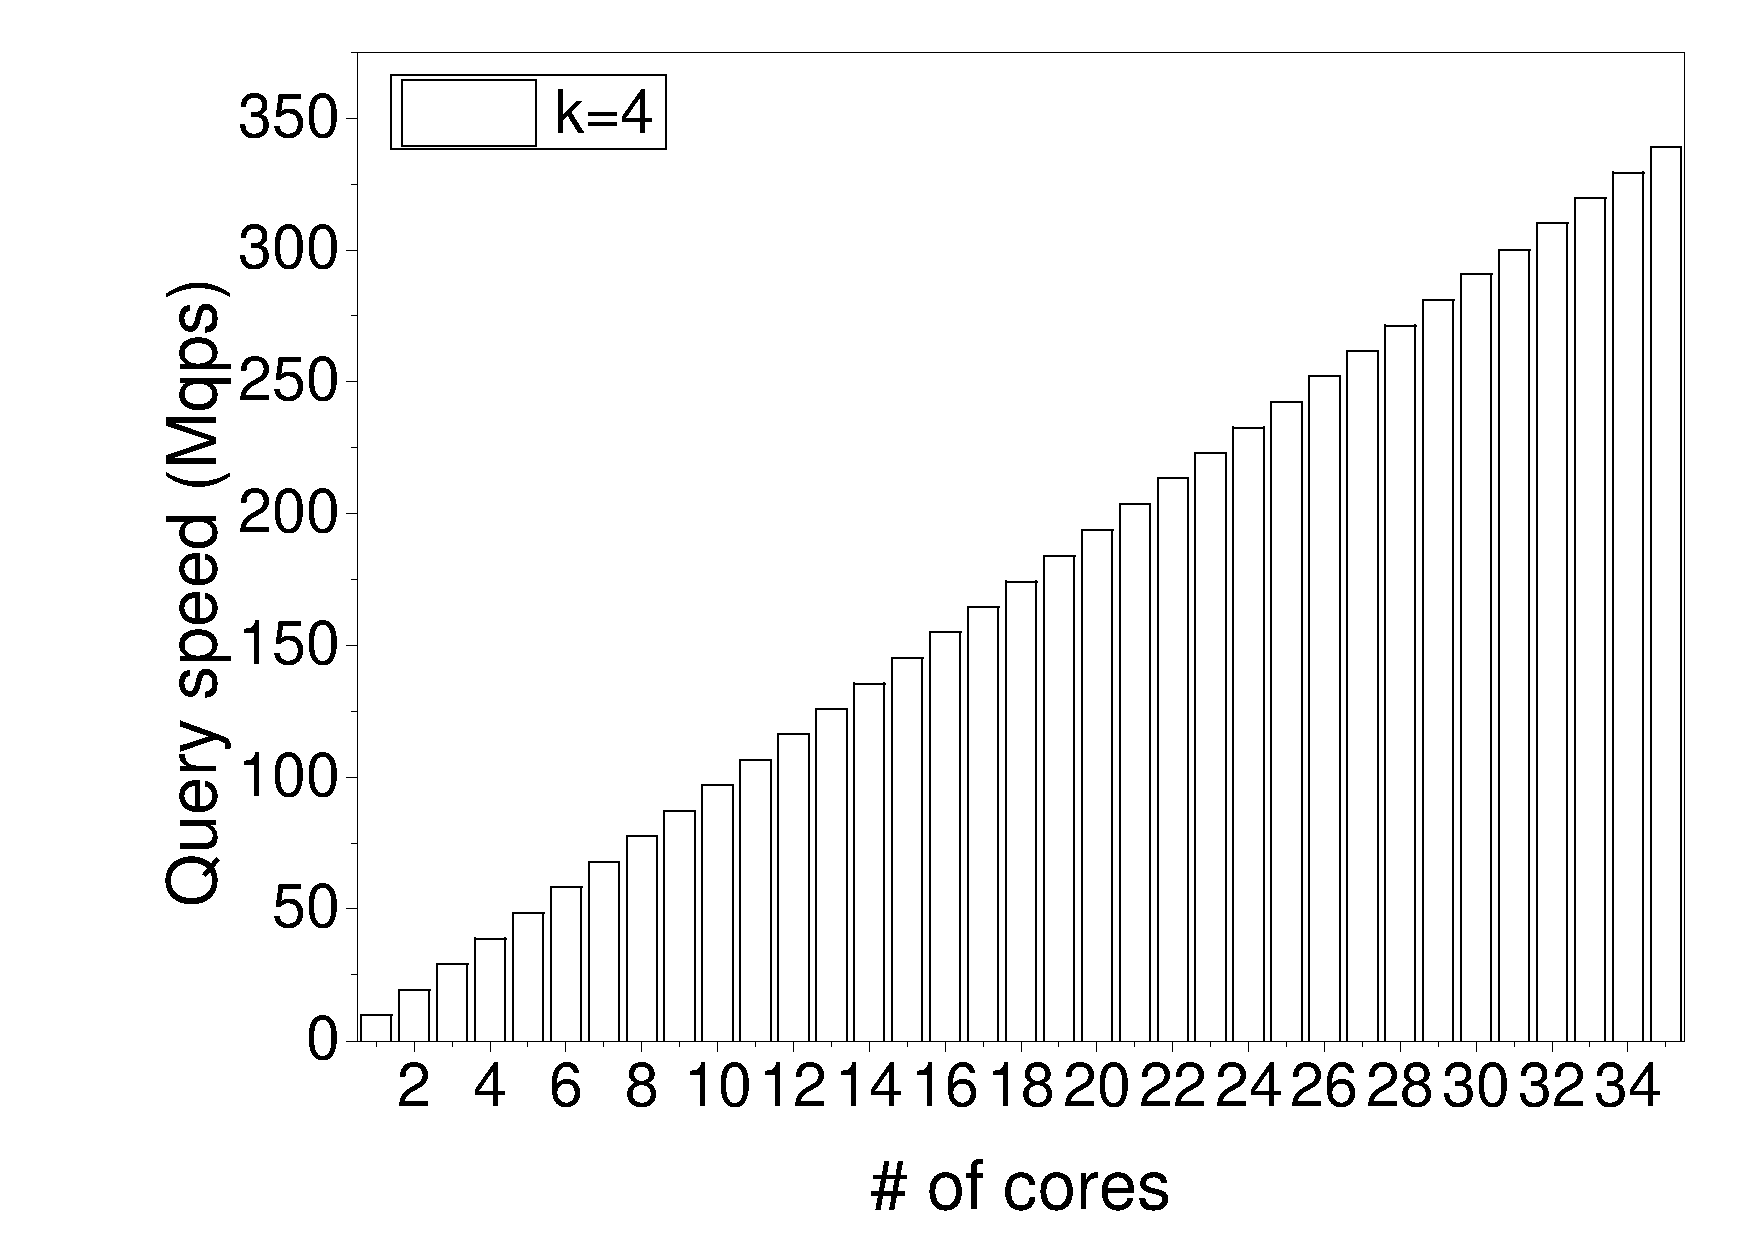
\includegraphics[width=6.2cm]{manyCoreTraffic1}}
 %		\centerline{(a) k=4}
 %	\end{minipage}
 %	\hfill
 %	\begin{minipage}{0.32\linewidth}
 %		\centerline{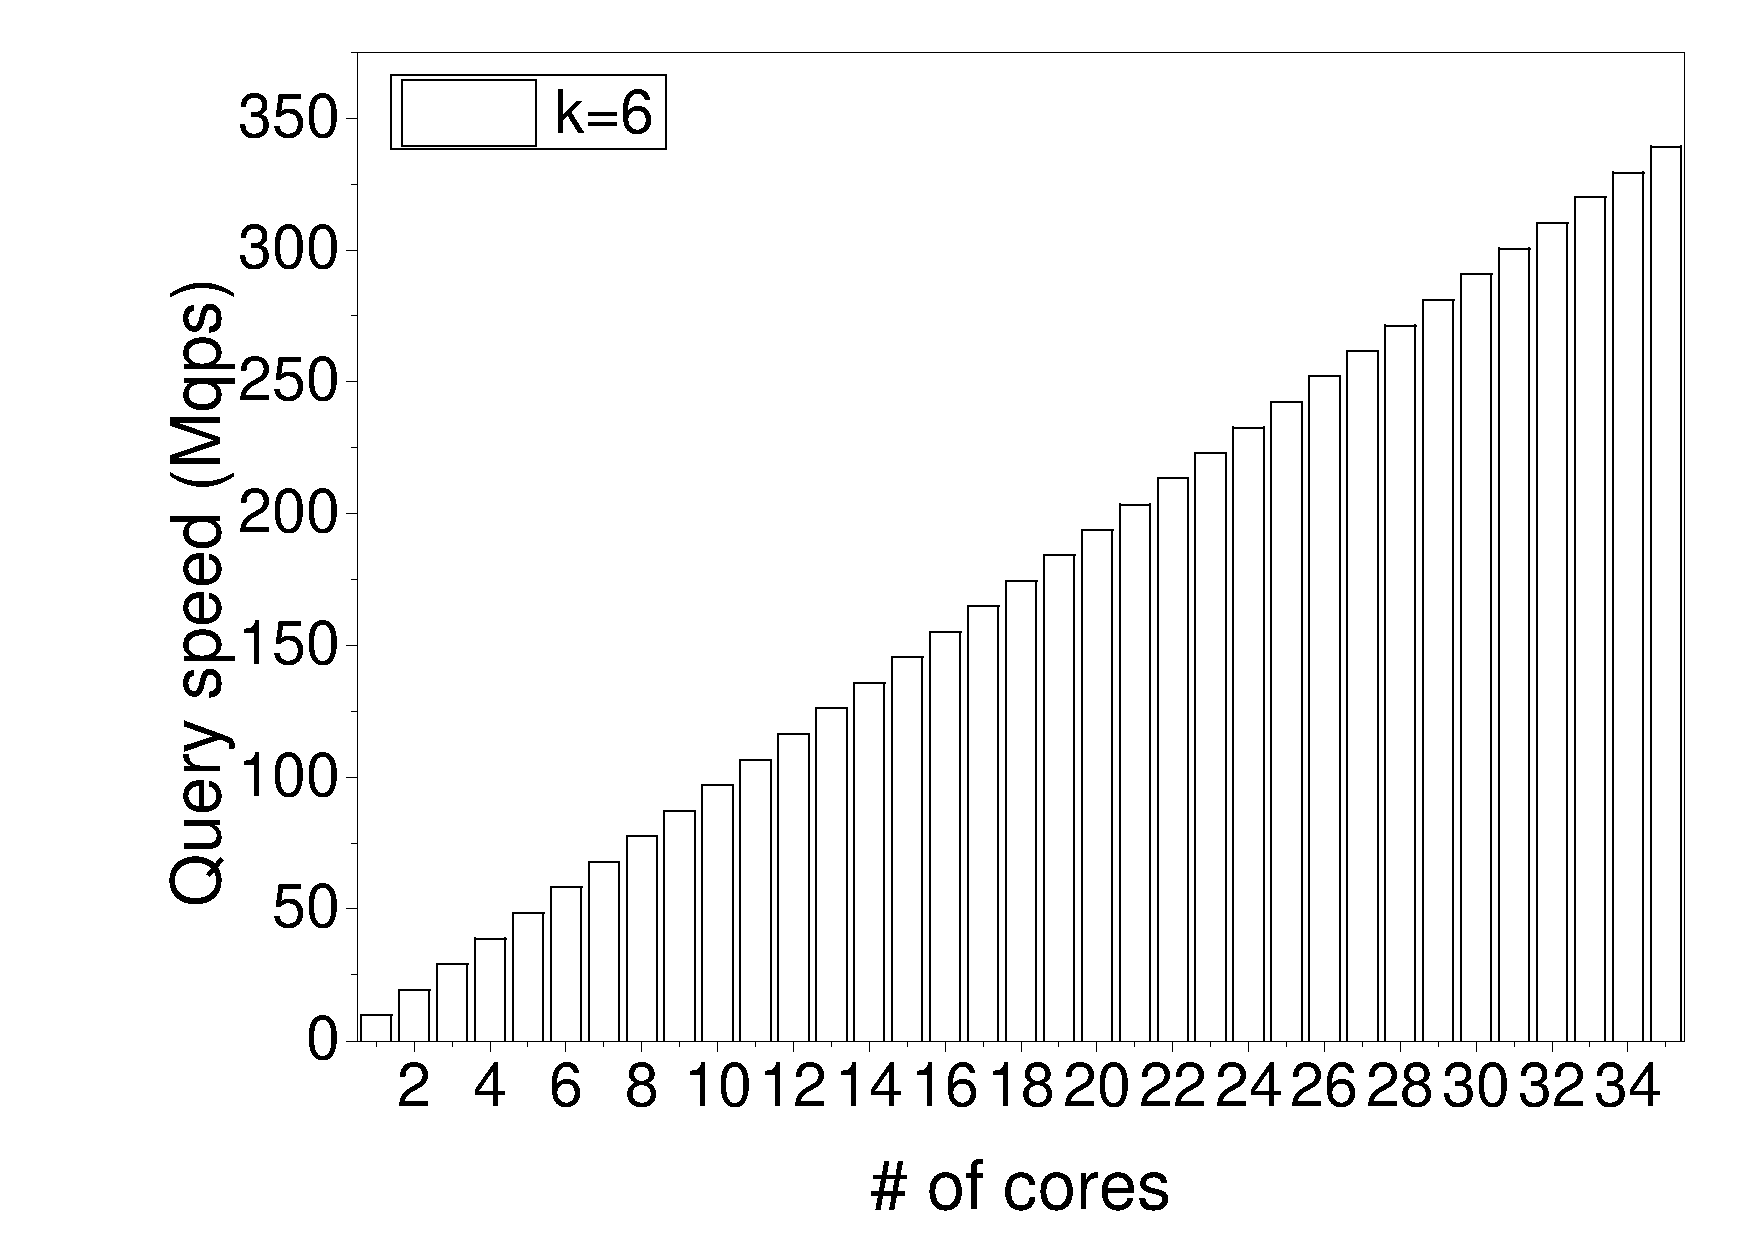
\includegraphics[width=5.8cm]{manyCoreTraffic2}}
 %		\centerline{(b) k=6}
 %	\end{minipage}
 %	\hfill
 %	\begin{minipage}{0.32\linewidth}
 %		\centerline{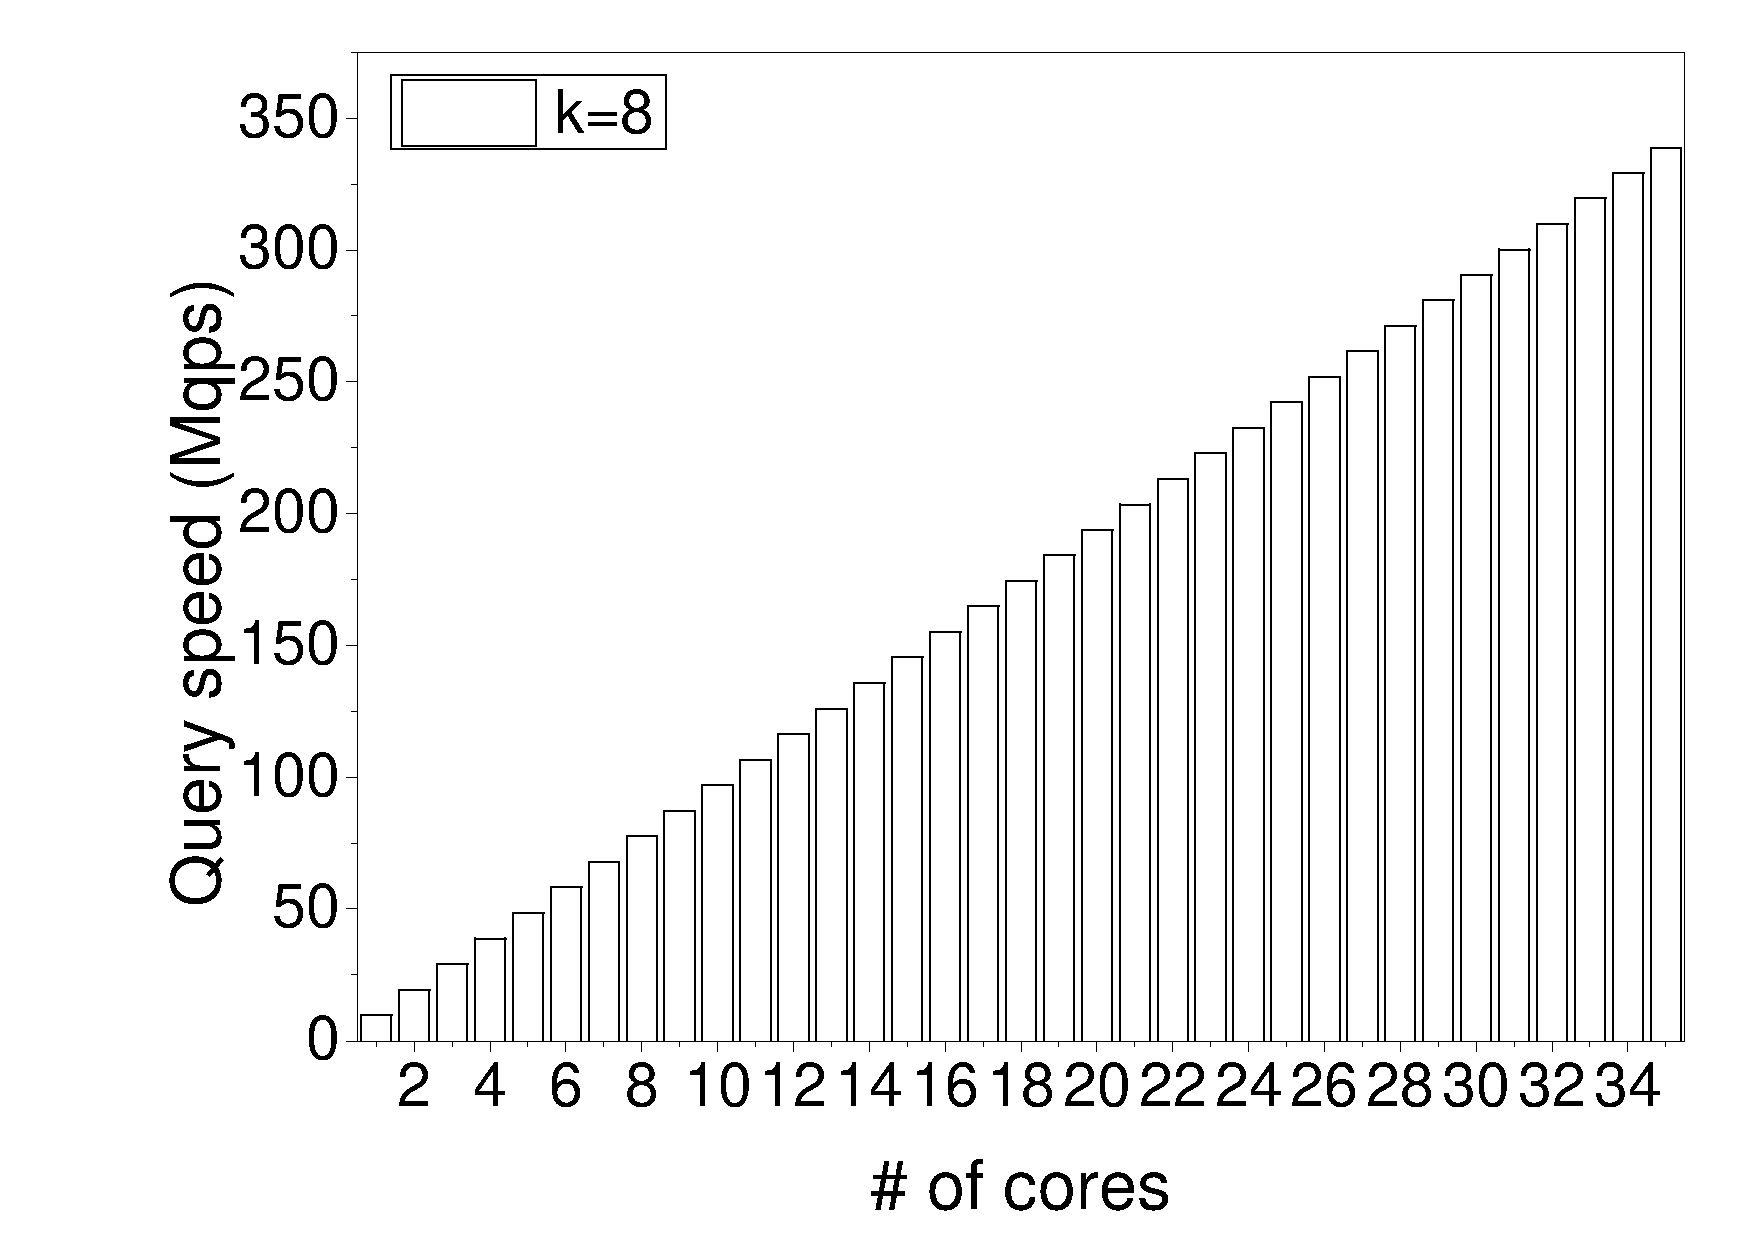
\includegraphics[width=5.8cm]{manyCoreTraffic3}}
 %		\centerline{(c) k=8}
 %	\end{minipage}
 %	\caption{Query speed VS. \# of cores.} \vspace{-0.1in}
 %	\label{fig:manycore:QPS}
 %\end{figure*}
 
We can see from the figure that the optimal $k$s are totally identical between the theoretical and practical results. For example, when $m=100,000$, $n=12,000$ and the best $k$ should be 5.78 obtained from the previous formula \ref{equ:mykform}. And because $k$ is an integer, so it should be 6. In our experiment, when $k$ is 6, the FP probability is the lowest, which is 1.816\% in the 15 spots ranging from 2 to 16. The same logical also applied to other cases when $n$ is 8,000 or 10,000.

%\presub
%\subsection{Performance Test on CPU and Many-core Platform} \postsub

 %To better understand the SBF, we conduct the performance test of SBF on two platforms: CPU and Many-core.

 %\subsubsection{Performance on CPU}

 %We run the program on the same computer described above in the experimental setup section. We set up the SBF with the parameter $n=5000$, $k=4,6,8$ respectively and $m$ to be optimal according to the formula \ref{formulaM}. Then we query 100,000,000 elements in the 100M-traffic file. And for each 1,000,000 queries, we sum up the running time and calculate the query speed. The 100 spots are showed in Figure \ref{fig:PC:QPS}. The average query speed is $13.068Mqps$ (Million queries per second) when $k=4$, $12.496Mqps$ when $k=6$, and $12.326Mqps$ when $k=8$.




 %\subsubsection{Performance on Many-core Platform}

 %We also evaluated the query speed on the SBF versus the number of cores. We carry out experiments on the many-core platform Telera TLR4-03680. The many-core processor has 36 cores with a 256K L2 cache for each one. One L2 cache access needs 9 cycles. 

 %In our implementation of the C++ program on many-core platform, we set one core to serve as the main thread and all other 35 cores to be the query threads. Also the main thread is in charge of dividing and distributing 35,000,000 elements (also from the beginning of the 100M traffic file) to 35 groups. Each group has 1,000,000 elements to be queried by one core and each core has its own SBF instance for querying. Of course, the SBF instances in the 35 cores are exactly the same with each other. We set up the SBF with the parameters $n=5000$, $k=4,6,8$ respectively and $m$ to be optimal according to the formula \ref{formulaM}.

 %Our experimental results are showed in Figure \ref{fig:manycore:QPS}. We can see that as the number of cores grows, the query speed increases linearly. Note that because one core is responsible for the main thread, which distributes the elements and collects the results from other cores, we only have the results of 35 cores. And the query speed can achieve $339Mqps$ when $k=4$ and 35 cores are running in parallel.







